
 
% # •••••••••••••••••••••••••••••••••••••••••••••••••••••••••••••••••
% Comparing the Simulated Elections with US Congressional Elections (PA)
% =================================================================
% -- FIGURE -- FIGURE -- FIGURE -- FIGURE -- FIGURE -- FIGURE --   % 
% ----------------------------------------------------------------- 
\begin{figure}
    \begin{center}
    \caption{Comparing the Simulated Elections with US Congressional Elections (PA)}
    \label{fig:densityplots_congressional}
    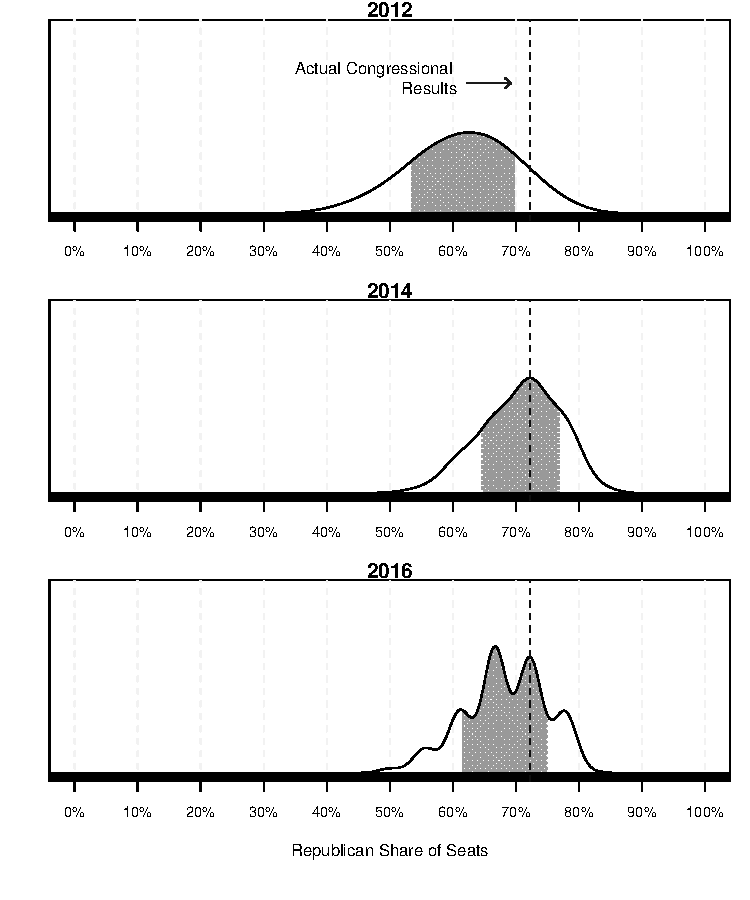
\includegraphics[width=1\textwidth]{Figures/fig_sims_actual_density.pdf}
    \end{center}
    \tabnotes{Plots based on the 2016 Five Election Composite data centered at the vote share for each year. All percentages in terms of Republican share of the two-party vote from the composite measure of five state-wide races in 2016. Shaded area contains one standard deviation on either side of the mean, representing 68\% of the simulated seat percentages.}
\end{figure}
% -----------------------------------------------------------------
% -- END FIGURE -- END FIGURE -- END FIGURE -- END FIGURE -- END FI %
% =================================================================
 